\chapter{Attacks and vulnerabilities}
\label{ch:attacks_vulnerabilities}
This chapter reviews the main sources of vulnerabilities and attacks, from Kerckhoffs' principle to \sout{hackers} attackers.

%----------------------------------------------------------------------------------------

\section{Kerckhoffs’ principles}
\textbf{Auguste Kerckhoffs}, a Netherlands born cryptographer, wrote in his 1883 essay \textit{La Cryptographie Militaire} six principles of practical cipher design:

\begin{enumerate}
    \item The system should be, if not theoretically unbreakable, unbreakable in practice.
    \item \textbf{The design of a system should not require secrecy, and compromise of the system should not inconvenience the correspondents.}
    \item The key should be memorable without notes and should be easily changeable.
    \item The cryptograms should be transmittable by telegraph.
    \item The apparatus or documents should be portable and operable by a single person.
    \item The system should be easy, neither requiring knowledge of a long list of rules nor involving mental strain.
\end{enumerate}

In spite of being more than 130 years old, some of these principles still hold.

%----------------------

\subsubsection*{First principle}
An evergreen. It is ok if our cryptographic system is not perfect; perfection is hardly achieved, and brute force attacks are always possible. However, any feasible attack should need too much time to be performed, in order to make eventual intel unneeded.

%----------------------

\subsubsection*{Second principle}
As already stated in section \ref{sec:internet_threat_model}, the most important among these six rules, simply called \textbf{Kerckhoffs’ principle}, is the second one, which in other words says that \textit{security by obscurity} is a very bad idea.

We should never employ an unnecessarily complicated system, because we must never rely on the fact that an attacker does not know how the system works (he/she might be an intern), and when information about the system's structure leaks it makes it go from secure to completely unsecure. Also, as security is to be found in the design, we cannot even change it very often.

\vspace{0.5em}

\emph{Example} During World War 2 the Germans used Enigma, an extremely complicated machine, to secure their communications. When the British found one of those machines - not even a full one, but a reduced version - they reverse engineered it and broke the whole cryptography system.

\vspace{0.5em}

\emph{Example} There are companies that only share certain parts of the datasheets of their devices, resulting in a documentation with missing pages. These pages, which usually contain cryptography algorithms or other sensible information, are provided to the customer only after signing a non-disclosure agreement. They can often be found on Russian websites, though (see fig. \ref{fig:pirate_free_things}). However, industrial systems can still rely on security by obscurity because they have armies of lawyers: if anyone breaks such a system they will have them knocking at their door in no time - and lawyers are way nastier than the poopoos, especially when the system-breaker is a regular person and not some large organization.

\begin{figure}[h]
    \centering
    
\includegraphics[scale=0.5]{img/pirate_free_things.png}
    \decoRule
    \caption{You know how this goes.}
    \label{fig:pirate_free_things}
\end{figure}

%----------------------

\subsubsection*{Third principle}
The security of a system lies in its key. This was a good principle 130 years ago, but nowadays it is not very relevant because tasks are done by computers, and they do not have any problems in memorizing long keys.

It is worth saying that the point of stealing account passwords is to create databases, with the idea to later use them in brute force attacks. Having a number, a letter and a special character in passwords is not a good idea anymore; it is not the length of the password that makes it strong, either: the password's strength relies in randomness, and in the fact that it should be unrelated to anything else in the same dictionary (also, do not use the same password for all sites).

%----------------------

\subsubsection*{Fourth principle}
Irrelevant in 2020.

%----------------------

\subsubsection*{Fifth principle}
Irrelevant in 2020.

%----------------------

\subsubsection*{Sixth principle}
Cryptography should not be rocket science from the point of view of the user.

%----------------------------------------------------------------------------------------

\section{Outsourcing}
\textbf{Outsourcing} is an agreement in which one company hires another company to be responsible for a planned or existing activity that is or could be done internally, and sometimes involves transferring employees and assets from one firm to another. 

Nowadays we are constantly outsourcing something (e.g. cloud systems); lots of systems and/or services (a network, storage, service, anything) have \textit{at least} three entities involved: a \textbf{service customer}, a \textbf{service provider} (which could also outsource to someone else) and a \textbf{network operator}.

The \textbf{service provider} operates the service and its components, which in turn use the network infrastructure to reach the customer.

The \textbf{service customer} can customize the service and its components according to the contract with the service provider (usually only in the framework given by the service provider). It uses the service, and is not interested in how the network works.

The \textbf{network operator} builds, maintains, and runs the network infrastructure, which must respect the Quality of Service\footnote{From the point of view of security, QoS also means that data should not pass through untrustable countries, like China.} required by each service. The network operator should not be involved with the service.

%-------------------------------------------

\subsection{Service Level Agreement}
The \textbf{Service Level Agreement}, or \textbf{SLA}, is a written contract which states the goals of a service, the penalties for not meeting them and the limits. In other words, it defines what we can expect from a service, so as security analysts, we must check if there is anything related to data breaches, security, cryptography and - of course - privacy.

\begin{figure}[h]
    \centering
    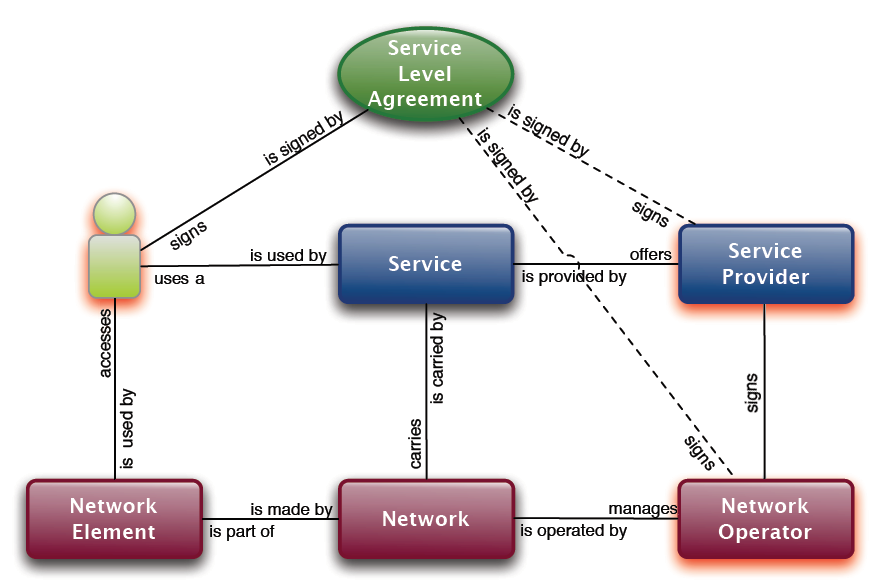
\includegraphics[scale=0.5]{img/sla.png}
    \decoRule
    \caption{Service Level Agreement diagram.}
    \label{fig:sla}
\end{figure}

The SLA is signed by the user (e.g. \textbf{EULA}, \textbf{End-User License Agreement}), and can be found between the user and the service provider. It is not uncommon, though, to have a SLA also between the service provider and the network operator, because if the latter is not involved in this agreement the security of a system cannot be fully enforced.

\subsubsection*{Vertical services}
It is much, much simpler if the service provider communicates with the network operator and tells them what kind of QoS or protection they need; this makes a service \textbf{vertical}.

A vertical service is bad for competition (thus a bad idea, especially in the long term), because whoever provides a service and has made an agreement with the network operator will have an advantage over his competitors.

\vspace{0.5em}

\emph{Example} We cannot watch Sky over a network that is not provided by Fastweb.

\vspace{0.5em}

%----------------------

\subsubsection*{Horizontal services}
If there is no SLA between the service provider and the network operator, then the diagram obtainable by modifying figure \ref{fig:sla} would be typical of \textbf{horizontal services}, like the ones built on the Internet. Here the customer can use a variety of services without knowing who their network operator is.

\vspace{0.5em}

\emph{Example} If we want to watch Hulu, Netflix, Sky, etc. we do not have to ask what is our network operator, we just go on the Internet and use them. If we use Outlook Mail but want to switch to Gmail, we can just change them.

\vspace{0.5em}

This scheme is good for competition, but since in horizontal services the network operator is not involved with the service provider, we must have a very good agreement with the network operator in order to get the best quality of service.

\vspace{0.5em}

\emph{Example} Suppose that we normally browse e-mails, but also and watch TV over Internet between 6 AM and 2 AM. We can tell the service provider what we are doing, but there is no way for us to ask the network operator for a larger bandwidth for movies (so as to adapt to the service that we are using in that moment). The network operator does not know what services we are using; it could, but it is not its job to do this: it is not interested in this, and even worse, we have to negotiate with them for good SLAs for our services.

\vspace{0.5em}

%----------------------

In cases where an extremely secure system is needed the rule of thumb is to not go towards full vertical services, but still sign a SLA between the network operator and the service provider. That is because in spite of, for example, a data center's security, the real problem lies in the transportation system, the network: an attacker is almost never close to source or destination, but is to be found somewhere in between.

%-------------------------------------------

\subsection{Hackers}
\begin{center}
\textit{A computer hacker is any skilled computer expert that uses their technical knowledge to overcome a problem. While "hacker" can refer to any skilled computer programmer, the term has become associated in popular culture with a "security
hacker", someone who, with their technical knowledge, uses bugs or exploits to break into computer systems.}
\end{center}

The term \textit{hacker} dates back to the 1960s, and is outdated;  per se, the term indicates somebody that hacks something else, or that is able to take a system, open it (physically), disassemble and reassemble it. Nowadays this word should \textit{never} be used, because it is way too generic for real security purposes. If somebody tells us that he/she has been attacked by hackers, they either have not been attacked at all or they have no idea of what that means.

In this section we will make a portrait of our attacker. In order to do this we must refer to the \textbf{hat color}, which gives a good characterization of the \textbf{purpose} of an attack (the one thing we are interested in).

The most dangerous attackers are the script kiddies, because they do not know what they are doing, while the most harmful ones are the black hats, because they \textit{do} know what they are doing. Finally, the most costly attackers are the white hats, because they will provide a long list of things to fix.

%----------------------

\subsubsection*{White hat attackers}
Their goal is to \textit{not} cause harm. These are the people who disassemble the system and tells us what is wrong with it.

%----------------------

\subsubsection*{Black hat attackers}
Their goal is to cause harm, possibly without leaving traces.

%----------------------

\subsubsection*{Grey hat attackers}
Things are not always black and white: these attackers are sometimes white, sometimes black.

%----------------------

\subsubsection*{Blue hat attackers}
These attackers are interns of a company, and work against a red team. The red hats work in security, while the blue ones try to break their system; in practice they are a sort of testers. White hats are sometimes called by companies to do this job.

%----------------------

\subsubsection*{Script kiddies}
\begin{center}
    \textit{Forgive them because they don't know what the fuck they're doing.}
\end{center}

While white and black hats tend to go against unknown/unusual vulnerabilities and are able to conceal themselves and not leave traces (at least not until it is too late), script kiddies, on the other hand, are those who use ready-to-make attacks (like the ones found on certain Linux distributions), without understanding the theory behind or even just what they are doing - or even if they do, they did not create their own tools.

Script kiddies (fig. \ref{fig:hackerman_attacks}) are the most common kind of attackers as well as the most dangerous, because they exploit known vulnerabilities that have been usually forgotten from patches and can unknowingly destroy important stuff while doing their thing.

Script kiddies are pretty much like mosquitoes: not very dangerous, but since there are many of them they are very annoying. Fortunately, they are preventable.

\begin{figure}[h]
    \centering
    
\includegraphics[scale=0.2]{img/hackerman.png}
    \decoRule
    \caption{This is what script kiddies think they look like (but they really don't).}
    \label{fig:hackerman_attacks}
\end{figure}

%----------------------

\subsubsection*{Hacktivists}
These attackers are extremely dangerous: they have a goal, a message to send to the world, and like anybody with a greater goal they do not think much about the real consequences of their actions.

\vspace{0.5em}

\emph{Example} People against the animal fur industry have found out that in a nearby town there is a place where animals are grown in order to be slaughtered for their fur. They go there and free those animals: they are hacktivist by all means, because they do no understand that in doing so they have released into the environment non-native animals which are not even used to live in the wild, resulting in a greater damage to the ecosystem.

\vspace{0.5em}

\emph{Example} A notorious group of hacktivists, Anonymous, started a campaign against pedophiles, and hacked pedophile websites and disrupted them. At a certain point the international police went to one of their spokespersons and asked them to stop, because in doing so they had deleted years of investigations aimed at jailing those people.

\vspace{0.5em}

Hacktivists have the means and the goals, but sometimes they cause significant side effects or, in some cases, they are plainly against the goal of somebody else (they want to impose their view to everybody else).

%----------------------

\subsubsection*{Nation states}
NSA and Israelian, Chinese, Russians, Italian Secret Services, etc. are all groups founded by governments, which have tools beyond our reach. Defending from any one of them is somewhat possible, but ultimately is not really effective: if they want it, they will break it. Also, there are a lot of nation state-sponsored hacking groups. Their attacks are possible, effective, and we will probably not be able to defend against them.

In a risk assessment for an industrial system we would have to consider them, but we could only pray to never have to cope with them; normally we would spend too much in order to defend against them, so we would simply not consider them at all.

%-------------------------------------------

\subsection{Vulnerabilities}
The only system without vulnerabilities is a computer which has been turned off and disassembled, and every part has been individually put in a different safe, each of which placed at different locations. In fact, even this might not be enough. 

There are no systems without vulnerabilities\footnote{There \textit{might} actually exist a few systems without vulnerabilities, but it could also be just a matter of time until somebody finds a bug in them, too.}, and any really secure system is a useless one (because it does not exist). Every application contains at least a bug and an instruction that could have been left out. By induction, all programs could be reduced to a single, \textit{wrong} instruction.

Vulnerabilities stem from many different reasons:

\begin{itemize}
    \item by \textbf{design};
    \item by \textbf{\textit{bad} design};
    \item by \textbf{\textit{bad} implementation};
    \item by \textbf{\textit{bad} deployment};
    \item by \textbf{library/OS update};
\end{itemize}

%----------------------

\subsubsection*{Vulnerabilities by design}
A \textbf{vulnerability by design}, as the name implies, arises from the way in which the system has been designed. In these cases the vulnerability is well known and accepted; the choice to allow such a flaw in the system is usually motivated by simplicity, compatibility and other similar reasons (in many cases the system would not work if the vulnerability would have been patched).

Examples of vulnerabilities by design include:

\begin{itemize}
    \item resource discovery protocols;
    \item ARP/NDP;
    \item NAT.
\end{itemize}

%----------------------

\subsubsection*{Vulnerabilities by \textit{bad} design}
A \textbf{vulnerability by \textit{bad} design} arises from a fundamental mistake or oversight in the software's design. Often these vulnerabilities are caused by badly implementing a standard. In these cases, even though the programmer pays attention to every single line of code, reads the documentation and does everything that is possible in order to avoid mistakes, more often than not it is the standard itself that is written in a dramatically obscure, unclear or even missing way. This is either because whoever wrote it did not realize that they did not explain it in a decent way, or because they intentionally wanted to give advantage to some implementers by leaving out fundamental details from the public standard and then giving them to a few chosen people (for commercial purposes; an example of this is the 5G standard, of which only those who contributed to it know all the details).

Examples of vulnerabilities by bad design include:

\begin{itemize}
    \item SAMBA (Windows file sharing);
    \item attacks on speculative executions in CPUs\footnote{Speculative execution is an optimization technique where a computer system performs some task that may not be needed.};
    \item errors in the management sequence for exceptions.
\end{itemize}

%----------------------

\subsubsection*{Vulnerabilities by \textit{bad} implementation}
There are \textbf{vulnerabilities by \textit{bad} implementation} because coders are underpaid, and because the release cycle of software is too fast. Programming done right would require two people in front of a monitor and full tests for every single test case, but companies are not willing to pay the price of making robust software, so nobody does that.

The only cases where software is super-checked is that of avionics systems (military aircrafts) - but even they could still contain important vulnerabilities (e.g. the Orion capsule failure\footnote{Orion (officially Orion Multi-Purpose Crew Vehicle or Orion MPCV) is a class of partially reusable space capsules to be used in NASA's human spaceflight programs. On November 30th, 2020, it was reported that NASA and Lockheed Martin had found a failure with a component in one the Orion spacecraft's power data units which casts uncertainty on a November 2021 launch date, since it could take months to fix.}).

There are countless examples of vulnerabilities by bad implementation, including:

\begin{itemize}
    \item incomplete if/then/else clauses;
    \item memory copies left unchecked;
    \item input left unchecked.
\end{itemize}

Countermeasures to this kind of vulnerabilities are writing tests and documentation, and giving implementers and coders enough time and resources to do a good job.

%----------------------

\subsubsection*{Vulnerabilities by \textit{bad} deployment}
\textit{Bad} deployment happens whenever we have foreseen an event in the design, but the people who deployed it did not read the docs and thus did not account for it. Basically, the system works just fine in the laboratory and test bed, but not on the field.

A possible countermeasure against this vulnerabilities is to, well, read the manual. Carefully.

%----------------------

\subsubsection*{Vulnerabilities by library/OS update}
These vulnerabilities are to be found not in the application itself, but in the libraries and/or the operating system it uses. They are more common than one might think.

Examples of library vulnerabilities include:

\begin{itemize}
    \item use of deprecated/obsolete functions (usually signalled by warnings at compilation time; deprecation means that that function has been found to be bugged and/or is not maintained anymore, and sometimes it might even be empty and only consist of a signature);
    \item random numbers actually not very random (correlation).
\end{itemize}

Countermeasures include containers and virtualization, which isolate the system.

\vspace{0.5em}

\emph{Example} If we are developing a Python application, we can use a virtual environment so that we can install new packages without messing up existing ones; we can develop and test the code by making sure that nothing, except ourselves (when updating an existing library or installing a new one), will ever mess up with the underlying system.

\vspace{0.5em}

%----------------------

\subsubsection*{More about vulnerabilities}
An alternative classification of vulnerabilities goes by \textit{"I know about it"} and \textit{"Oh shit, I didn't know about it"}.

Since vulnerabilities are extremely important, there are initiatives that pay people to find them (bug/vulnerability bounty, vulnerability hunting, etc.).

Finding new vulnerabilities, however, is not easy: we have to put the system in a controlled environment, test it, find any problem and then what vulnerability it leads to. The final prize then depends on how good was the report, if the vulnerability has already been reported, etc.; the reward for having found a vulnerability can go from the price of a pizza to that of a brand new car (even hundred of thousands of dollars, upfront cash).

There are entire databases of known vulnerabilities, among which the most important is the \textbf{CVE}, \textbf{Common Vulnerabilities and Exposures}\footnote{\url{https://cve.mitre.org/}}. It contains full descriptions and consequences of not patching a vulnerability of hundreds of past problems that afflicted software.

CVE is not meant to be a shame wall for companies that did something wrong\footnote{It actually is if the company has a long list of bugs but, yeah.}. It has been made in order to allow sysadmins to check if their system is vulnerable to something, and what are the countermeasures, which often are easier than patching or updating the whole thing (e.g. in big industries it is better having a known problem, one that we know how to avoid, rather than a system that does not have any problems but might have older ones that we do not know about). Vulnerabilities entered into the CVE attain to the ethics of white hat hacking, as CVE contains only patched bugs.

In general, the way of communicating a bug after finding it is fundamental. A white hat hacker writes a report, sends it to the relevant party and does his/her best to reach it until they give them feedback. In any case, the hacker cannot publish the vulnerability, unless either the company told him/her that they do not trust them or do not care, or he/she did not get an answer in a long time (from about six to nine months). A white hat hacker could also publish a vulnerability if they also found that it is actively being used in the wild, although this is a borderline case.